\chapter{Análisis de Resultados}
\label{ch:anarel}

En el presente capítulo se hará un análisis de los resultados obtenidos del SPDE. Partiremos revisando la importancia de las variables sobre el modelo de predicción, y además, comprobaremos algunas hipótesis basadas en la teoría que finalmente la evidencia empírica las confirmó. Finalmente, se señalará la relevancia de predecir la deserción, pues quizá es más interesante predecir el abandono, pues como se señaló en capítulos anteriores, la deserción es un proceso que se va desencadenando con varias etapas, una de ellas es un abandono por el alumno.

\subsection{Importancia de las variables o atributos}
Para poder analizar la importancia de las variables de entrada utilizadas en el modelo de predicción, es necesario utilizar un algoritmo de aprendizaje automatizado que le asigne pesos relativos a las variables. Lamentablemente el modelo de predicción creado en el Capitulo[cita] utiliza el algoritmo AdaBoost que no es capaz de señalar qué variables son más relevantes que otras. Como vimos anteriormente, el bosque aleatorio también era una opción viable, debido a la diferencia mínima con el algoritmo AdaBoost. El bosque aleatorio sí tiene la posibilidad de mostrar las importancias relativas de cada variable. Es precisamente por esto que desde ahora en adelante para efectos de este capítulo, utilizaremos un bosque aleatorio entrenado en la mismas condiciones que el capítulo citado anteriormente.
Si entrenamos un modelo de predicción utilizando la muestra de estudio y la totalidad de las variables seleccionadas obtenemos los resultados de clasificación en el conjunto de entrenamiento y de prueba se muestran en la Figura~\ref{fig:clas-total}.
\begin{figure}[H]
  \centering
    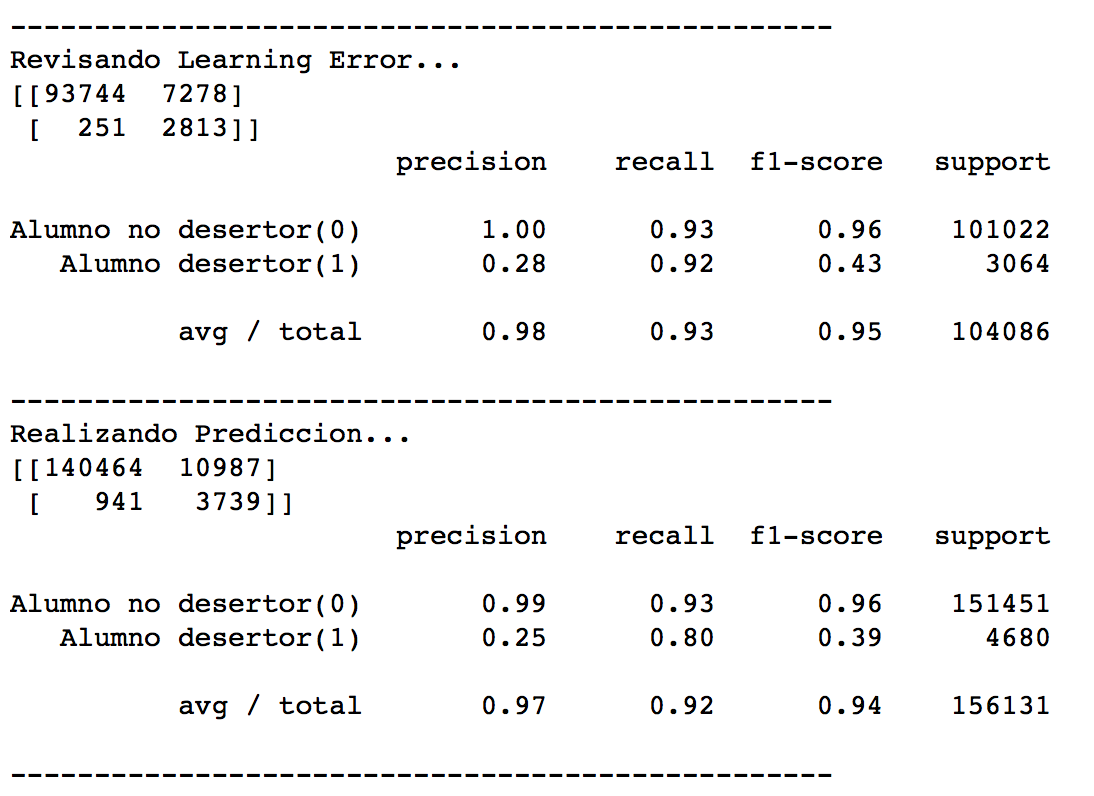
\includegraphics[trim=0cm 0cm 0cm 0cm,scale=0.65]{Figuras/7AnalisisResultado/clas-total.png}
      \caption{Reporte de clasificación del modelo de predicción utilizando Bosques Aleatorios con todas las variables disponibles}
    \label{fig:clas-total}
\end{figure}
Además en la Figura~\ref{fig:impo-total} vemos los atributos que mejor discriminan los datos utilizando el algoritmo de bosques aleatorios. Al revisar esta información, podemos ver que los atributos más importantes son la sobre edad del alumno, percentil del alumno en el curso del promedio general y de la asistencia. Mientras que también son importantes, pero en menor medida, la escolaridad superior de los padres y otras características del establecimiento al que asiste.
\begin{figure}[H]
  \centering
    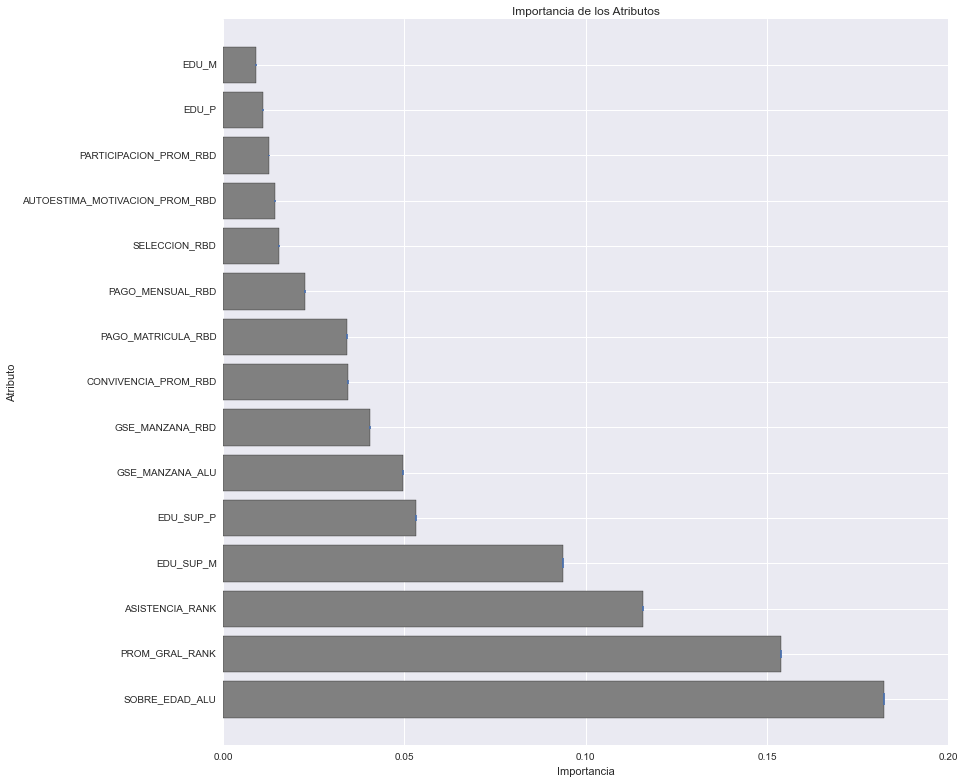
\includegraphics[trim=0cm 0cm 0cm 0cm,scale=0.4]{Figuras/7AnalisisResultado/impo-total.png}
      \caption{Importancia de las variables de entrada del modelo de predicción utilizando Bosques Aleatorios con todas las variables disponibles}
    \label{fig:impo-total}
\end{figure}
Ahora nos preguntamos, por qué estas variables tienen un buen poder discriminatorio para poder detectar casos de deserción y el algoritmo de aprendizaje automatizado le asigna menor importancia a la demás variables que son también, en base a la literatura, cruciales para detectar alumnos en riesgo de deserción. Esto ocurre por que existe una relación dependiente entre el promedio general, la asistencia y la sobre edad con la demás variables. Es decir, estas variables contienen toda la información anterior. Esto era un resultado esperable, ya que en experiencias anteriores se ha visto que se puede predecir, con muy buen poder de clasificación, la deserción escolar utilizando solamente estas variables. El problema de utilizar estas variables en el modelo es que, si bien son capaces de almacenar todo lo que le ocurre al alumno, no dan luces de la razón de por qué el alumno va a desertar, que finalmente, esto es lo que importa, pues así se pueden alinear fácilmente los programas de intervención. La única ventaja que tiene esto es que es muy fácil obtener esta información desde el MINEDUC. En base a esto, se puede plantear en el futuro, desarrollar un modelo de predicción utilizando todos los datos históricos de los promedios generales y la asistencia.Pero, lamentablemente, esta información es de carácter auto-reportada y los establecimientos tienen grandes incentivos para manipular esta información[cita], por tanto, tampoco son indicadores muy confiables.

Dicho lo anterior, ahora procederemos a eliminar las variables que poseen la mayoría de la importancia, es decir, la sobre edad, el percentil del promedio general y la asistencia con la finalidad de evaluar el poder de explicación del modelo de predicción, pues como dijimos anteriormente, explicar la deserción sería muy interesante para las tomares de decisión. Los resultados de la predicción en el conjunto de prueba se pueden ver en la Tabla~\ref{fig:clas-parcial} y la importancia en la Figura~\ref{fig:impo-parcial}.
\begin{figure}[H]
  \centering
    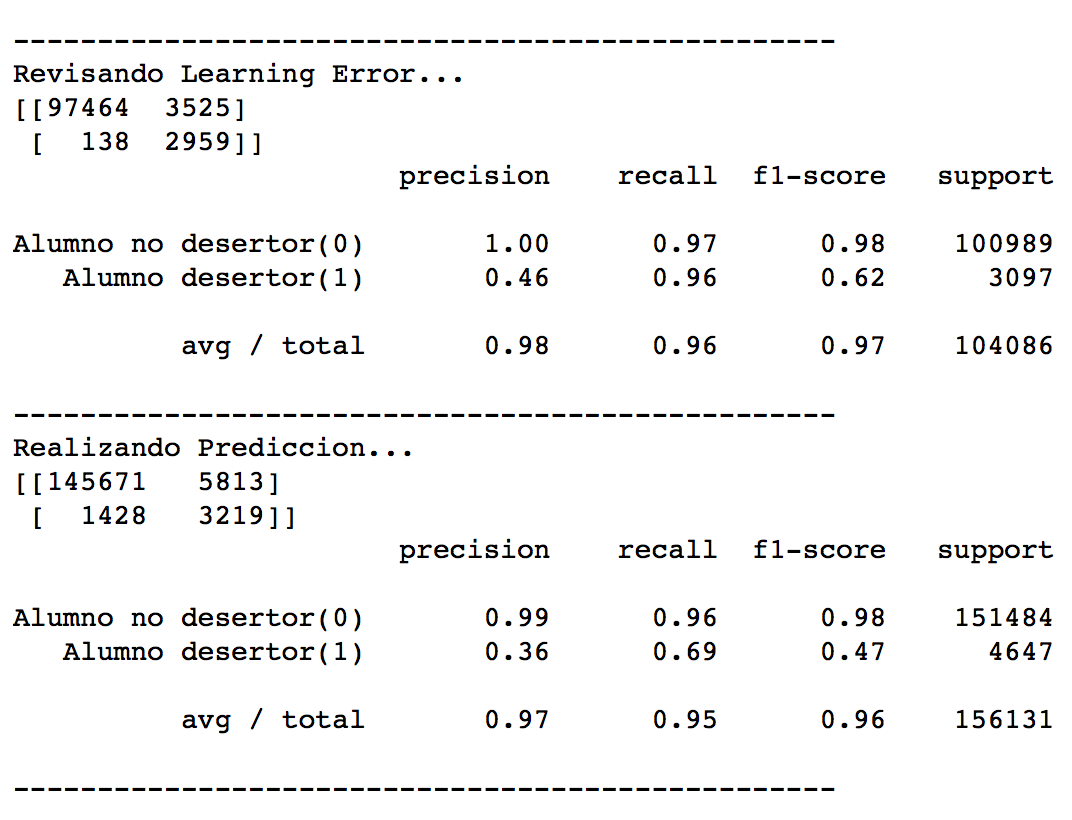
\includegraphics[trim=0cm 0cm 0cm 0cm,scale=0.65]{Figuras/7AnalisisResultado/clas-parcial.png}
      \caption{Reporte de clasificación del modelo de predicción utilizando Bosques Aleatorios sin las variables de sobre-edad y percentiles del promedio general y asistencia}
    \label{fig:clas-parcial}
\end{figure}
Al ver las importancias relativas de cada atributo podemos ver que ahora el protagonismo lo tienen las variables de la información de la educación superior de los padres y el grupo socioeconomico de barrio del alumno y en menor medida, el grupo socioeconomico del barrio del establecimiento. Si nos fijamos en estos resultados, en conjunto con el poder de clasificación, vemos que baja el poder de clasificación y se cumple nuevamente la misma estructura anterior donde existe un quiere de la importancia al tener 3 variables. 
\begin{figure}[H]
  \centering
    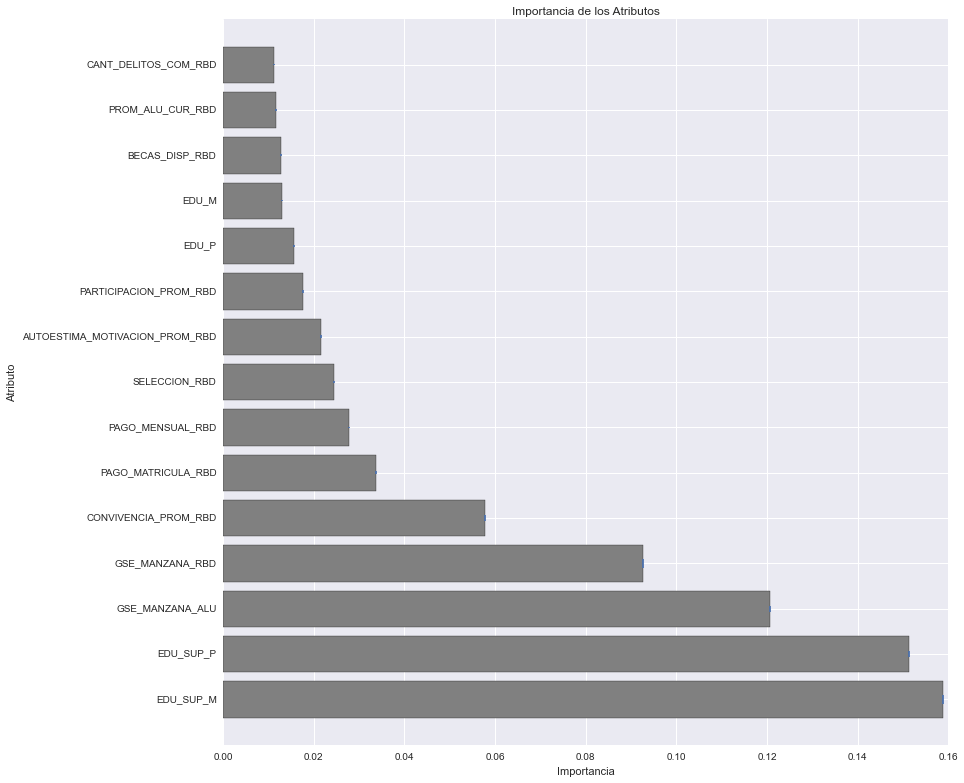
\includegraphics[trim=0cm 0cm 0cm 0cm,scale=0.4]{Figuras/7AnalisisResultado/impo-parcial.png}
      \caption{Importancia de las variables de entrada del modelo de predicción utilizando Bosques Aleatorios sin las variables de sobre-edad y percentiles del promedio general y asistencia}
    \label{fig:impo-parcial}
\end{figure}

Esto nos señala que, efectivamente, el promedio general, la asistencia y la sobre edad, poseen mucho más de información que las variables mostradas en la Figura~\ref{fig:impo-parcial}. También señala que como no bajó el poder de clasificación significa mente, se cumple la hipótesis de qué la sobre edad, el percentil del promedio general y la asistencia son linealmente dependientes de las demás variables y por esto que el algoritmo les da mayor importancia a estas. Podríamos considerar redundante las variables señaladas en la Figura~\ref{fig:impo-parcial}.
Ahora si analizamos la capacidad explicativa del modelo de predicción anterior, notamos que la variables que más importan son variables, prácticamente, de largo plazo y muy difíciles de intervenir. Por ejemplo, la escolaridad superior de los padres no es algo que se pueda cambiar, pues ya es demasiado tarde en el momento que el modelo muestra estas razones como explicaciones a la deserción. Ocurre lo mismo con el grupo socioeconomico, pues como este es el grupo socioeconomico del barrio, estos raramente cambian al corto plazo.

Finalmente, otro análisis interesante está en evaluar la importancia de los atributos separadamente por educación básica y media. En la Figura~\ref{fig:clas-basica} y Figura~\ref{fig:clas-media} se encuentran los reportes de clasificación utilizando los datos de solamente la educación básica y media respectivamente. Al comparar ambas figuras podemos ver que para la educación media la importancia son las mismos, pero estos difieren en magnitud. Lo que podemos ver es que el grupo socioeconomico del barrio del alumno, sube en magnitud y aporta casi al mismo nivel que si los padres poseen eduacción superior. De esto se puede desprender de que en la educación media los alumnos están en un periodo de edad donde obtienen mayor independencia en su vida, por tanto, es muy importante el barrio por donde transita. Además, existe una hipotesis[cita] que se señala que, en general, en los sectores de grupos socioeconomicos bajos, existe mayor delicuencia en estos. Aquí también puede haber una mayor importancia entre grupo socioeconomio del barrio del alumno y lo que ocurre allí para detectar casos de deserción escolar en estudiantes de educación media.

\begin{figure}[H]
  \centering
    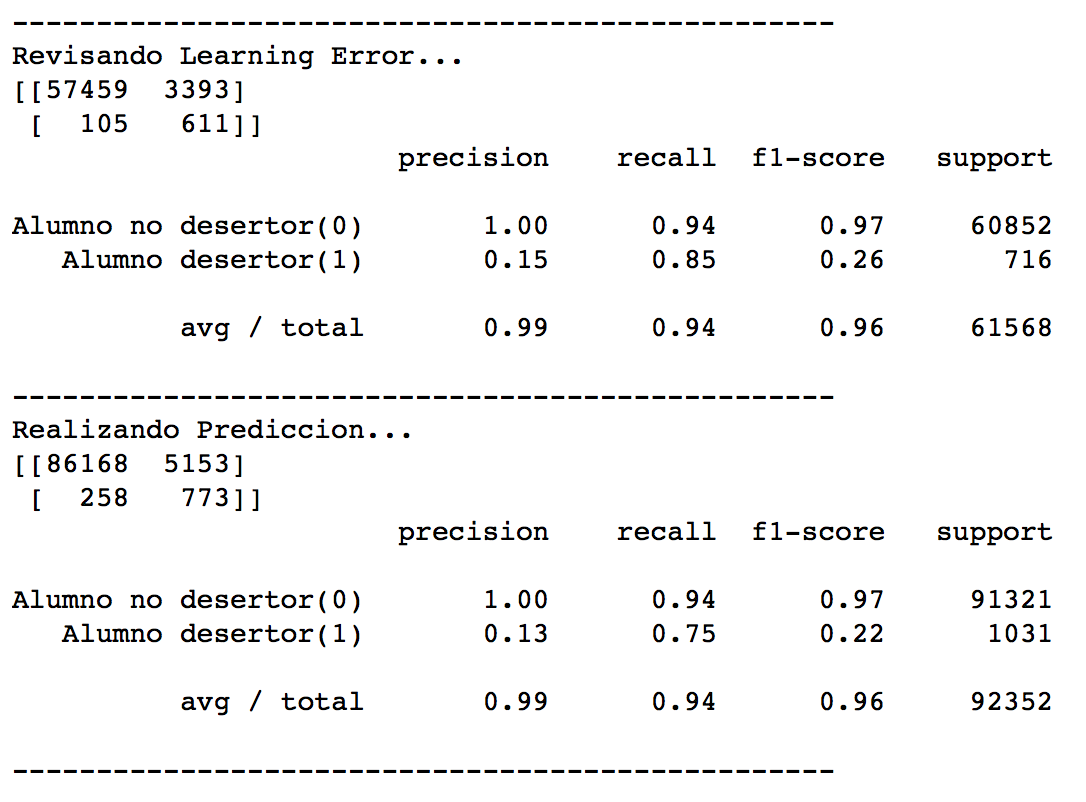
\includegraphics[trim=0cm 0cm 0cm 0cm,scale=0.65]{Figuras/7AnalisisResultado/clas-basica.png}
      \caption{Reporte de clasificación del modelo de predicción utilizando Bosques Aleatorios de la educación básica sin las variables de sobre-edad y percentiles del promedio general y asistencia}
    \label{fig:clas-basica}
\end{figure}
\begin{figure}[H]
  \centering
    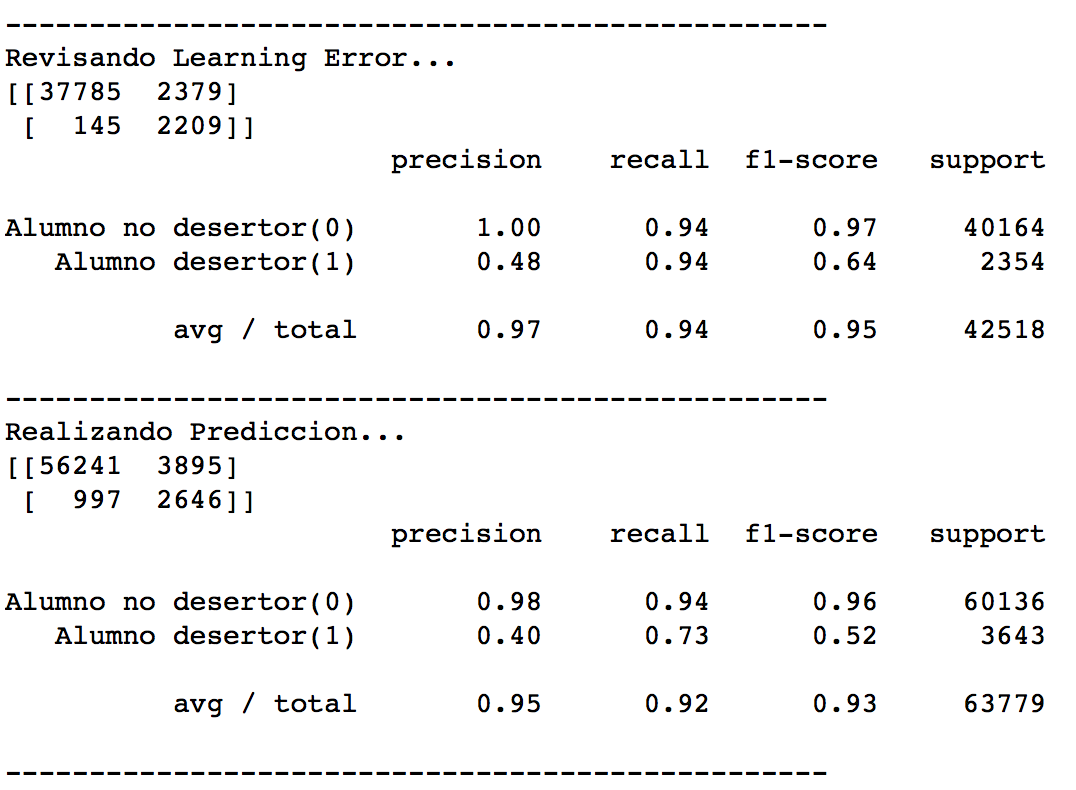
\includegraphics[trim=0cm 0cm 0cm 0cm,scale=0.65]{Figuras/7AnalisisResultado/clas-media.png}
      \caption{Reporte de clasificación del modelo de predicción utilizando Bosques Aleatorios de la educación media sin las variables de sobre-edad y percentiles del promedio general y asistencia}
    \label{fig:clas-media}
\end{figure}

Además, en la Figura~\ref{fig:impo-basica} y Figura~\ref{fig:impo-media} la importancia de las variables en educación básica y media respectivamente.

\begin{figure}[H]
  \centering
    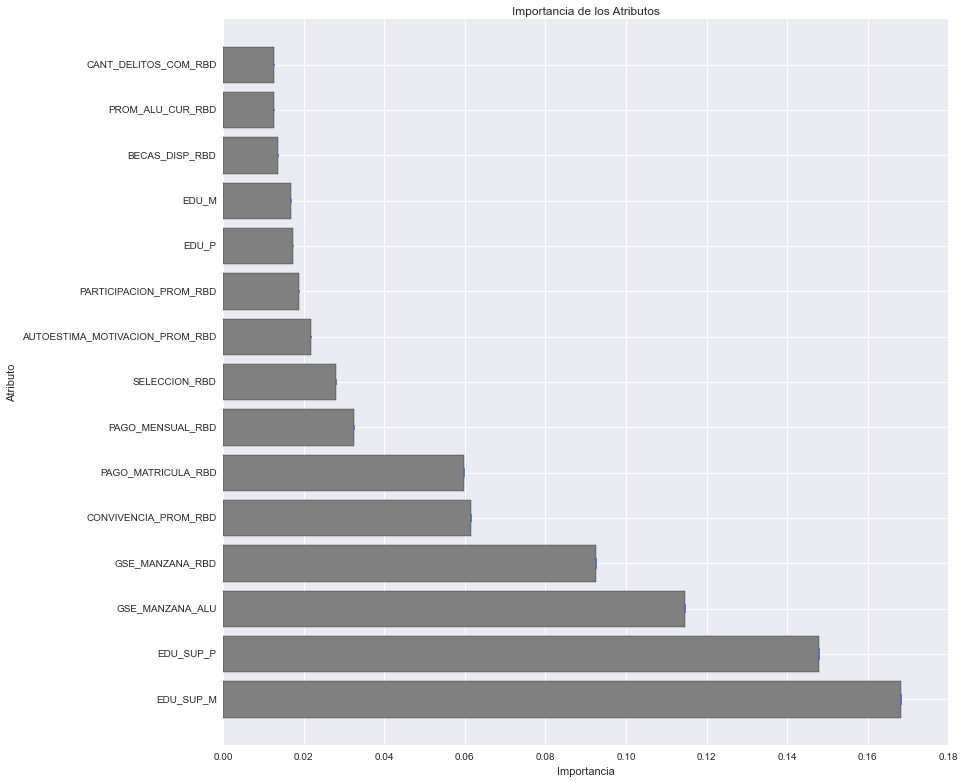
\includegraphics[trim=0cm 0cm 0cm 0cm,scale=0.4]{Figuras/7AnalisisResultado/impo-basica.png}
      \caption{Importancia de las variables de entrada del modelo de predicción utilizando Bosques Aleatorios de la educación básica sin las variables de sobre-edad y percentiles del promedio general y asistencia}
    \label{fig:impo-basica}
\end{figure}

\begin{figure}[H]
  \centering
    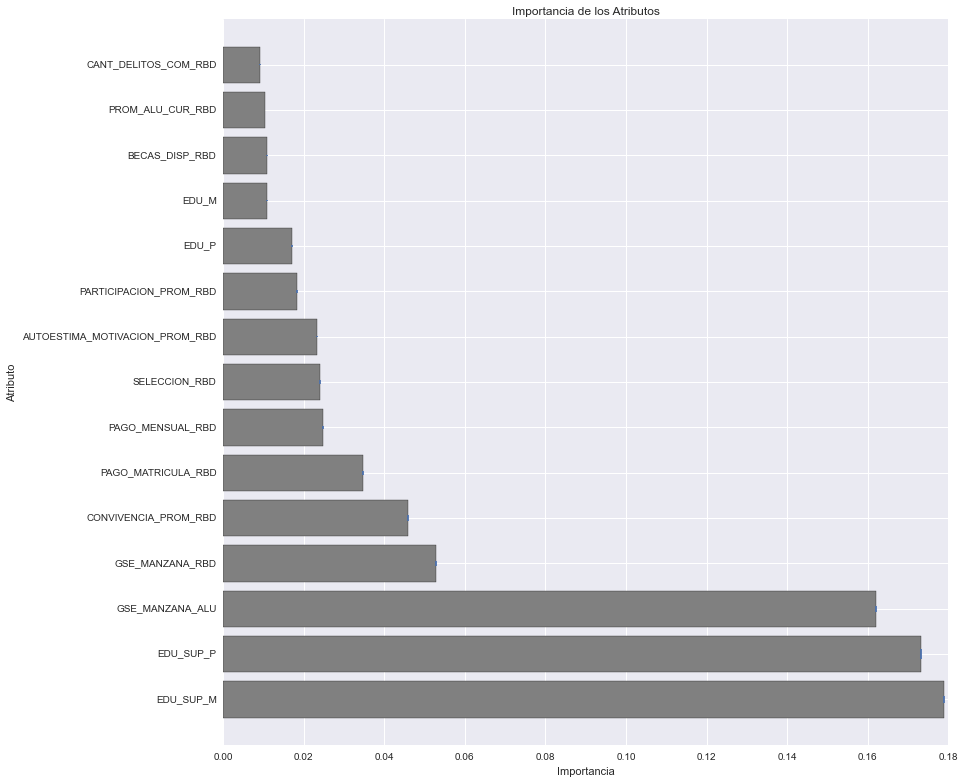
\includegraphics[trim=0cm 0cm 0cm 0cm,scale=0.4]{Figuras/7AnalisisResultado/impo-media.png}
      \caption{Importancia de las variables de entrada del modelo de predicción utilizando Bosques Aleatorios de la educación media sin las variables de sobre-edad y percentiles del promedio general y asistencia}
    \label{fig:impo-media}
\end{figure}